\documentclass[10pt,a4paper]{article}
% usepackages
\usepackage[utf8]{inputenc}
%\usepackage[latin1]{inputenc}
\usepackage[english]{babel}
% math
\usepackage{amsmath}
\usepackage{amsfonts}
\usepackage{amssymb}
\usepackage{mathtools}
\usepackage{latexsym}
% formatting
\usepackage{parskip}
\usepackage{fullpage}
\usepackage{pgf,tikz}
\usepackage{mathrsfs}
\usetikzlibrary{arrows}
\usepackage[round]{natbib}
%\pagestyle{empty}
% graphics
%\usepackage[pdftex]{graphicx}
\usepackage{caption}
\usepackage{subcaption}
%\usepackage[below,section]{placeins} % the one below is better for short assignments
\usepackage{float} % provides H as float placement specifier
% extras
\usepackage[pdftex,a4paper,colorlinks=true,urlcolor=blue]{hyperref}
\urlstyle{same}
\usepackage{moreverb} %\verbatimtabinput{filename.py} preserves indentation

%Numbering first level list roman (i,ii,iii) instead of arabic (1,2,3)
% options are \roman \Roman \alph \Alph \arabic
%\renewcommand{\theenumi}{\roman{enumi}} 
%\renewcommand{\theenumii}{\roman{enumii}}
%\newcommand{\Int}{\int\limits}
\pagenumbering{arabic}
% Also achieved with the enumerate package
\usepackage{enumerate}
%\numberwithin{equation}{section}%

% author/title details
%\author{Alice NANYANZI (\href{mailto:alicenanyanzi@aims.ac.za}{alicenanyanzi@aims.ac.za})}
% \title{Course Title: Assignment X}
%\theoremstyle{plain}
\newtheorem{thm}{Theorem}

%\theoremstyle{definition} 
\newtheorem{defn}{Definition}
\newtheorem{exa}{Example}


\title{Technical Report}
\date{\today}
\begin{document}
	\maketitle
	
	\vspace{1cm}
	\section*{Outline}
	\section{Diffusion on networks}
	\subsection{Motivation}
	Diffusion on networks is one of the dynamic processes that occur on networks. Diffusion processes on networks are used to develop models for the study of real-world processes such as the spread of infections with in a group of people, spread of information in a social network, studying failures in power supply on the grid with in an area, etc.
	\subsection{Ideas}
	\begin{enumerate}[a)]
		\item  Diffusion on networks through direct interactions
		\item  Accounting for long-range interaction in diffusion process on network
		\item k-path Laplacians, that is, the generalised Laplacian matrices. Considerations of Mellin and Laplace transforms of the k-path Laplacians to account for longrange interactions
		\item Illustration of Diffusion of heat on a lattice. First, considering direct interactions only and then accounting both direct and long-range interactions. 
	\end{enumerate}
    \section{Image Segmentation}
    \subsection{Motivation}
    Image Segmentation is the problem of localising regions of an image relative to content. It aids in the extraction of objects of interest from an image. Image segmentation has applications in medical field, engineering field, computer science among others. A number of segmentation techniques have been developed based on graph theory concepts which include intelligent scissors, Normalised cut algorithm, random walker algorithm, etc. Our interest is in the segmentation of images using the random walk process on graph as put forward by Grady.
    \subsection{Ideas}
    \begin{enumerate}[a)]
    	\item To extend the idea of image segmentation using random walks on networks by accounting for long-range links in the network. Our aims is to ascertain whether a better image segmentation can be obtained on including long-range links.  
    \end{enumerate}
    \section{Systemic Risk and Contagion in Financial Systems}
    \subsection{Motivation}
    The financial crisis of $2008$ stimulated intense research in the area of financial systems. The use of complex networks in the study of financial systems is one of the avenues that have been used by a number of research in uncovering the root causes of the crisis, which financial institutions sparked off the cascaded failure leading to system break down, the impact of the network structure, strategies to  either prevent the re-occurance or to guarantee minimal impact of the crisis etc. 
    \subsection{Ideas}
    \begin{enumerate}[a)]
    	\item The concept of "too interconnected to fail",i.e which measure (centrality) can we use to identify nodes that are considered too interconnected to fail.
    	\item Can the centrality based on generalised degree centrality capture the node which is too interconnected to fail?
    	\item How can we apply the concept of long-range interactions to financial networks? What does the long-range interactions mean?
    \end{enumerate}
	\section{Laplacian centrality of an edge}
	\subsection{Motivation}
	Centrality measures in networks have proved to be relevant tools in network analysis. They are indicators of the 'importance' of nodes and edges in the networks. Though most work has been geared towards the study of importance of nodes ( i.e degree, closeness, betweeness, subgraph, eigenvector, Laplacian centralities,etc.), interest in the study of edge centralities is now gaining ground with prominent works of  Girvan and Newman. some of the known edge centralities include edge-betweenness, k-path edge centrality, among others. The motivation for the introduction of edge centrality measures lies in real-world applications in a wide range of context such as in identifying communities in networks, identifying strong relationships among people in social networks, etc. 
	\subsection{Ideas}
	\begin{enumerate}[a)]
		\item Extend the concept of Laplacian centrality of  nodes to edges, obtain the graph theoretical description of the edge centrality.
		\item What is the relation between Laplacian centrality of the node and that of an edge?
		\item Can we apply the concept of edge centrality to the minimum cut problem in graphs?
		\item Yang et.al, in his work "Air traffic network optimization via Laplacian energy maximization" highlights the change in Laplacian energy due to edge removal as a promising fair measure of network robustness. We consider comparing this measure with other measures of network robustness.
		\item How can we apply the edge laplacian centrality to the concept of robustness in targeted edge attacks
		\item Application of laplcaian centrality of an edge to edge consensus, that is, addition or removal of edges so the relative difference in centrality of edges is small.
		\item Application to electric flow in circuits
	\end{enumerate}
	
	\section{Minimum-maximum cut}
	\subsection{Motivation}
	The minimum cut of a network is the minimum weight or number of edges whose removal results into a disconnected network. The max-flow min-cut theorem states that in a flow network, the maximum amount of flow passing from the source to the sink is equal to the total weight of the edges in the minimum cut, i.e. the smallest total weight of the edges which if removed would disconnect the source from the sink. This theorem has applications in image segmentation, and in optimisation problems such as project selection by guiding the decision regarding the purchase of machines that can be used in a number of projects so as to maximise profits of the company.
	\subsection{Ideas}
	\begin{enumerate}[a)]
	\item Investigate whether there exists a unique feature or behaviour for the nodes around the minimum cut.
	\item Whether the minimum cut edges can be obtained by their Laplacian centrality.
	\item  relation between Laplacian energy and the minimum cut of a network.
	\end{enumerate}
	\section{Noise on networks}
	\subsection{Motivation}
	In systems made of interconnections of sensors, it's observed that the reported results from  the systems are normally subject to errors due to noise. In order to obtain accurate results, we need to ascertain the effect of noise on the reported results. Since these systems can be represented as networks, we can then formulate this problem as one of studying the impact of noise on sensor network. 
	\subsection{Ideas}
	\begin{enumerate}[a)]
		\item How do we define noise on networks? Could the noise be applied to nodes or edges? 
		\item What could be the effect of noise on the structure of a network
		\item What insights do we draw from simulation of noise on networks by considering additive White Gaussian noise for instance?
	\end{enumerate}
	
	\section{Communicability in Networks}
	\subsection{Motivation}
	Communicability in networks in a concept introduced by Estrada \& Hatano based on the motivation that most real networks, communication between nodes does not necessarily follow shortest paths only as normally assumed. Evidence shows that communication can occur along any paths which are not shortest path. Communicability between a pair of nodes accounts for all possible walks through which a given pair of nodes can communicate. Some of the applications of this concept include community detection in networks. We are looking forward to research possibilities in this area which include the following:
	\subsection{Ideas}
	\begin{enumerate}[a)]
		\item Consider the impact of long range interactions to communicability in networks
		\item Other possible real-world application of communicability in networks
	\end{enumerate}
	
	
	%\section{Consensus in Networks}
	%\subsection{Motivation}
	%\subsection{Ideas}
	
	\newpage
	\section*{Work Progress}
    \section{Diffusion on networks}
    Diffusion is, among others, the movement of substance from a region of high concentration to a region of low concentration. Such substance include heat, gas, etc. \citep{newman2010networks}.
    
    Diffusion process over networks is one of the methods used in developing simple models that depict the spread of infections in a population, dissemination of information over social network for instance social network marketing, spread of heat over a conductor, among others. A number of models based on diffusion process have been developed and documented in \citep{estrada2011epidemic,kasprzak2012diffusion,lopez2008diffusion}.
    
    \subsection{Heat Diffusion Models}
    In this work, we consider spread of heat on a network. Recently, various models have been developed to depict the spread of heat heat diffusion process on networks which include selection of marketing candidates in social network marketing, data analysis and processing in which the observed data is considered as a sum of diffusion processes, dimensionality reduction and classification problems   \citep{ma2008mining,thanou2017learning,belkin2003laplacian}.
    
    Let us consider a simple example illustrating the diffusion process on a simple network. Let $G=(V,E)$ be a simple connected undirected graph with vertex set $V$ and edge set $E$. Suppose we randomly select a few nodes ( that is, sources) to which we assign specific amounts of heat as in vector $\phi_0$. With the heat diffusion coefficient, $C \in [0,1]$ which controls the rate of diffusion. When $C$ tends to $0$, heat transfer among nodes becomes difficult and as a result, heat does not spread to each of the nodes with in the network. However, as $C$ tends to $1$, heat spreads rapidly among nodes and thus, with out loss, heat is distributed to all nodes in the network.
    
   At each time $t$, we obtain the quantities of heat at each node, $\phi_t$. The spread of heat is considered to occur following the edges connecting nodes, that is to say, through direct interactions.  
%     We then try to understand how the heat will spread through out the network, whether equilibrium can be attained and if so, when does this happens?? We then explore the impact of network structure and node centralities on heat diffusion.
%    \begin{enumerate}[a)]
%    	\item Direct interactions
%    	Let us consider a simple network where a few randomly selected nodes are assigned quantities of heat $\phi_i$. The diffusion process is considered to occur by means of interactions between neighbouring nodes in the network. This mode of interaction is referred to as direct interactions. 
    	
    	The process of heat spread through out the network can therefore be modelled by
    	\begin{equation}
    	\frac{d\phi_i}{dt} = C \sum_j (\mathbf{A}_{ij} - \delta_{ij} k_i) \phi_j,
    	\label{difusion}
    	\end{equation}
    	where $\mathbf{A}$ is the adjacency matrix, $k_i$ is the degree of node $i$, and $\delta_{ij}$ is the Kronecker delta whose value is $1$ if $i=j$ and $0$ otherwise. In matrix-vector notation, we have
    	\begin{equation}
    	\frac{d\boldsymbol{\phi}}{dt} = -C\mathbf{L}\boldsymbol{\phi}, \quad \boldsymbol{\phi}(0) = \boldsymbol{\phi}_0 ,
    	\label{dif-final-eqn}
    	\end{equation}
    	whose solution is 
    	\begin{eqnarray}
    	\boldsymbol{\phi}(t) = \boldsymbol{\phi}_0~e^{-C\mathbf{L}t}.
    	\end{eqnarray}
    	Alternatively, the solution can be expressed as a linear combination of eigenvectors of the Laplacian matrix. That is
    	 \begin{eqnarray*}
    	 	\boldsymbol{\phi}(t) = \sum_i \langle \boldsymbol{\phi}(0),\mathbf{v}_i \rangle \quad e^{-C\lambda_i t} \mathbf{v}_i,  
    	 \end{eqnarray*}
    	 where $\lambda_i$, $\mathbf{v}_i$ are respectively the eigenvalues and corresponding eigenvectors of the Laplacian matrix and $\langle \boldsymbol{\phi}(0),\mathbf{v}_i \rangle$ is simply the projection of $\boldsymbol{\phi}(0)$ onto the set of eigenvectors.
    	 
    	 \subsection{ Equilibrium behaviour }
    	 As $t$ goes to infinity, we have 
    	 \begin{equation}
    	 \lim_{t \to \infty} e^{-C\lambda_i t} = \begin{cases} 0 &\mbox{if } \lambda_i > 0 \\
    	 1 & \mbox{if } \lambda_i = 0, \end{cases} 
    	 \end{equation}
    	 Asymptotically, the equilibrium state is completely determined by the kernel of $\mathbf{L}$. Since $\sum_{j} \mathbf{L}_{ij}=0$, it is easy to see that $\mathbf{v^1}= \frac{1}{\sqrt{n}}[1,\cdots,1]$, the eigenvector associated with $\lambda_i =0$, is in the kernel of $\mathbf{L}$. We then have
    	 %$\displaystyle \lim_{t \to \infty}\boldsymbol{\phi}(t)$, $a_i(t) = a_i(0) e^{-C \lambda_i t}$ where $\lambda_i = 0$. Since $L(\mathbf{v^1}) = \mathbf{0}$, for a given initial condition $\mathbf{a}(0)$ for a network with $n$ nodes, we have
    	 \begin{equation}
    	 \lim_{t \to \infty}\boldsymbol{\phi}(t) = \langle \boldsymbol{\phi}(0), \mathbf{v^1} \rangle \mathbf{v^1}.
    	 \end{equation}
    	 The quantity of heat $\phi_j(t)$ at any node $j$ at time $t$ is given by
    	 \begin{equation}
    	 \lim_{t \to \infty}\phi_j(t) = \frac{1}{n} \sum_{i = 1}^n \phi_i(0). 
    	 \end{equation}
    	 At steady state, the value of $\boldsymbol{\phi}$ converges to the same value at each of the nodes in the network, which is the average of the initial values at all of the nodes. This is because, as expected, neighboring nodes in the network will exchange heat until all nodes attain equal amounts of heat.
    	 
    	 For better understanding of the heat diffusion model, let us consider the following simple example.
    	 
    	 \begin{exa} Let us consider diffusion of heat over the network in Fig.~\ref{graph-plot}(\subref{difn-graph}). Suppose the quantity of heat at each node at time $t=0$ is given by the vector $\boldsymbol{\phi}(0)= [0.3,0.0,0.8,0.0,0.5,0.2,0.0,0.0,0.0,0.2]$, random values between $0$ and $1$. Let $C=0.05$. Fig.~\ref{graph-plot}(\subref{difn-plot}) illustrates how heat spreads over the network in Fig.~\ref{graph-plot}(\subref{difn-graph}). 
    	 	
    	 	\begin{figure}[!h]
    	 		\centering
    	 		\begin{subfigure}[b]{0.29\textwidth}
    	 			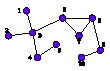
\includegraphics[width=\textwidth]{images/diffusion-graph.pdf}
    	 			\caption{}
    	 			\label{difn-graph}
    	 		\end{subfigure}~
    	 		\begin{subfigure}[b]{0.45\textwidth}
    	 			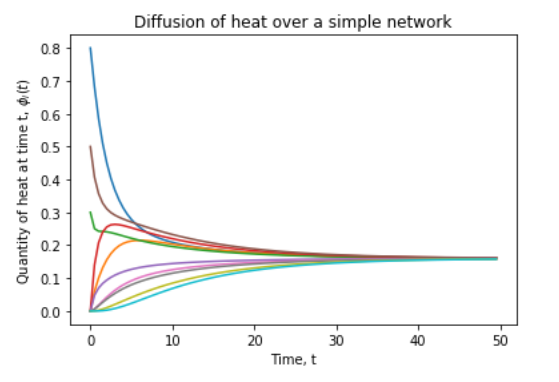
\includegraphics[width= \textwidth]{images/Diffusion-on-network-new.png}
    	 			\caption{}
    	 			\label{difn-plot}
    	 		\end{subfigure}
    	 		\caption{(\subref{difn-plot}) is an illustration of the diffusion process over the network in (\subref{difn-graph}). }
    	 		\label{graph-plot}
    	 	\end{figure}
     	  We observe that at each time step $t$, nodes that initially have high amounts of heat (i.e $1,3,5,6,$ and $10$) exchange heat with adjacent nodes that initially had none or little amounts of heat. The latter gain heat from the former and eventually all nodes in the network have relatively equal amounts of heat. This explains the fact that as time $t$ increases, the quantity of heat $\boldsymbol{\phi}_j(t)$ at each node tends to the equilibrium value of $0.2$.  From the fig, we can observe a tendency to equilibrium at around $t=35$. 
    	 \end{exa}
        
         
        \subsection{Diffusion on Directed Networks}
        A directed graph, also known as a Digraph or directed network, is one in which all the edges are directed from one vertex to another. 
        
        There are various complex systems whose skeleton can be captured by directed networks. Examples include ecological  networks, power grids, transportation networks, communication networks, metabolic networks, gene regulatory networks, citation networks among others. It is therefore paramount to study how dynamic processes such as diffusion, consensus, occur on such networks.
        
        \begin{defn}[Strongly connected Digraph]
        	A digraph is called strongly connected if and only if any two distinct nodes of the graph can be connected via a path that respects the orientation of the edges of the digraph \citep{saber2003agreement}.
        \end{defn}        
        For a strongly connected digraph with atleast two distinct nodes and with no self loops, the diffusion process on this network can be modelled in a similar manner as its undirected counterpart by 
        \begin{equation}
        \frac{d\boldsymbol{\phi}}{dt} = -C\mathbf{L}\boldsymbol{\phi}, \quad \boldsymbol{\phi}(0) = \boldsymbol{\phi}_0.
        \end{equation}
        For undirected graph $G$, the graph Laplacian,$L$, is symmetric positive semi-definite. However, for directed graphs $L$ is non-symmetric which implies that the diffusion on the former and latter graphs is not necessarily the same.
        
        \subsection{Equilibrium behaviour in Directed Network}
        In order to understand the process of attainment of steady state in networks, we need to study the spectral properties of graph Laplacian. Let $G=(V,E)$ be a digraph with Laplacian $L(G)$ with eigenvalues $\lambda_1, \lambda_2, \cdots, \lambda_n$ in non-decreasing order. 
        \subsubsection{Estimation of Eigenvalues of the Laplacian}
        Let $d_{max}$ be the maximum node out-degree of $G$, then following from Gershgorin disk theorem, then all the eigenvalues of $L(G)$ are located in the following disk
        \begin{equation} 
        D(G) = \{ z \in \mathbb{C} : |z-d_{max}| \leq d_{max} \}
        \end{equation}
        with centre at $z = d_{max} +0j$ in the complex plane \citep{saber2003agreement}. Thus, for a strongly connected digraph $G$, $L$ has a zero eigenvalue $\lambda_1=0$ and all the other non-trivial eigenvalues have non-negative real parts.
        Let us consider a strongly connected digraph $G=(V,E)$. Let $\boldsymbol{\phi}_0$ be the vector of quantities of heat at all nodes at $t=0$, $C=1$ be the diffusion coefficient. Similar to undirected case,the quantities of heat, $\boldsymbol{\phi}(t)$ at each node at a given time $t$ is given by
        \begin{equation}
        \boldsymbol{\phi}(t) = \boldsymbol{\phi}_0~e^{-\mathbf{L}t}.
        \end{equation}
        
        \begin{thm}[Limit Theorem for Exponential Matrices]
        	Assume $G$ is a strongly connected digraph with Laplacian $mathbf{L}$ satisfying $\mathbf{L} \mathbf{v_r} = \mathbf{0}$, $\mathbf{v_{l} ^T} \mathbf{L} =\mathbf{0}$, and $\mathbf{v_{l} ^T} \mathbf{w_r}=1$. Then 
        	
        	\begin{equation}
        	 R = \lim_{t \longrightarrow +\infty} exp(-Lt) = v_r  v_{l} ^T ]in M_n,
        	\end{equation}
        	where $M_n$ denotes a set of square $n\times n$ matrices, $v_r$,and $v_{l} ^T$ denote the right and left eigenvalues of $L$ associated with eigenvalue $\lambda_1 = 0$ \citep{saber2003agreement}.
        \end{thm}
    From the theorem, we deduce the for a strongly connected digraph, equilibrium state can be attained and the quantity of heat at the nodes is given by
    \begin{equation}
    \lim_{t \longrightarrow \infty} =  \boldsymbol{\phi}_0  \mathbf{v_r}  \mathbf{v_{l} ^T}
    \label{equildirected}
    \end{equation}
    It is important to note that following Equation \ref{equildirected}, any equilibrium value $x^*$ can be attained such that $x^*_i =x^*_j$ for all $i$, $j$. This therefore draws to find out which classes of digraphs attain equilibrium similar to that of undirected graphs where the value at each node is the average of the initial values at all nodes in the network.
    \subsubsection{Equilibrium state for Balanced Graphs}
    \begin{defn}[Balanced Graphs]
    	We say the node $v_i$ of a digraph $G=(V,E)$ is balanced if and only if its in-degree and out-degree are equal, that is, $d_{out}(v_i) =d_{in}(v_i)$. A graph $G$ is balanced if and only if all its nodes are balanced, i.e $\sum_j a_{ij} = \sum_j a_{ji}, \forall i$. 
    \end{defn}
     The proposition in \citep{saber2003agreement} states that 
     
     Let $G=(V,E)$ be a digraph with an adjacency matrix $A=[a_{ij}]$ satisfying $a_{ii}=0, \forall i$. Then, all the following statements are equivalent:
     \begin{enumerate}
     	\item $G$ is balanced,
     	\item $\mathbf{v_l}= \mathbf{1}$ is the left eigenvector of the Laplacian of $G$ associated with the zero eigenvalue, that is, $\mathbf{1}^T \mathbf{L} = 0$.
     	\item $\sum_{i=1} ^ n u_i = 0, \forall x \in  \mathbb{R}^n$ with $u_i = \sum_{j \in N_i} a_{i,j} (x_j -x_i).$
     \end{enumerate}
    
    
    	\subsection{ k-path Laplacian matrices}
    	
    	The k-path Laplacian matrices are a natural generalisation of the combinatorial Laplacian of a graph. The entries of these matrices are accounts of the existence of shortest paths of length $k$ between two nodes.
    	
    	The $k$-path laplacian matrix $\mathbf{L}_{k} (k \leq d_{max})$ of a connected undirected graph $G=(V,E)$ is defined as the square symmetric $n\times n$ matrix whose entries are given by:
    	\begin{equation}
    	\mathbf{L}_k(i,j) =  \begin{cases*}
    	-1 & if  $d_{i,j} = k,$  \\
    	\delta_{k}(i) & if $i = j,$ \\
    	0 & otherwise.
    	\end{cases*}
    	\label{kpathlap}
    	\end{equation}
    	
    	where $d_{i,j}$ is the shortest path distance between nodes $i$ and $j$, $delta_{k}(i)$ known as the $k$-path degree is the number of irreducible shortest paths of length $k$ having node $i$ as an endpoint.
    	
    	The concept of $k$-path Laplacians defined in Equation \ref{kpathlap} for finite undirected graphs was extended for connected and locally finite infinite graphs as follows:
    	Consider $\Gamma = (V,E)$ to be an indirected finite or infinite graph with vertices $V$ and edges $E$. We assume that $\Gamma$ is connected and locally finite that is to say each vertex has only finitely many edges emanating from it. Let $d$ be the distance metric on $\Gamma$, i.e. $d(v,w)$ is the length of the shortest path from $v$ to $w$, and let $\delta_{k}(v)$ be the $k$-path degree of the vertex $v$, i.e.
    	\begin{equation}
    	\delta_{k}(v) := \#\{w \in V : d(v,w) = k\}.
    	\end{equation}
    	Since $\gamma$ is locally finite, $\delta_{k}(v)$ is finite for every $v \in V$. Denote by $C(V)$ the set of all complex-valued functions on $V$ and by $C_{0}(V)$ the set of the complex-valued functions on $V$ with finite support. Moreover, let $\ell^2(V)$ be the Hilbert space of square-summable functions on $V$ with inner product
    	\begin{equation}
    	\langle f,g\rangle = \sum_{v\in V} f(v) \overline{g(v)}, \quad f,g \in \ell^2(V) 
    	\end{equation}
    	In $\ell^2(V)$ there is a standard orthonormal basis consisting of the vectors $e_v, v\in V$, where
    	\begin{equation}
    	e_v(w) :=  \begin{cases*}
    	1 & if  w = v,  \\
    	0 & otherwise.
    	\end{cases*}
    	\end{equation}
    	Let $\mathbf{L}_{k}$ be the following mapping from $C(V)$ into itself:
    	\begin{equation}
    	(\mathbf{L}_{k}) (f) := \sum_{w\in V: d(v,w)=k} (f(v) -f(w)), \quad f \in C(V).
    	\label{infinite-dif}
    	\end{equation}
    	
    	\subsection{Diffusion on network with long-range interactions (generalisation of diffusion equation on Graphs) }
    	
    	   	In this case, we consider diffusion on a graph where by both direct and long range interactions are involved. One interesting study of long range interactions is by Estrada on modelling epidermic spread in networks. Here, the long range interactions are considered to be nonrandom and depend on the social distances between individuals in the social network.
    	    Recently, Estrada introduced a method of generalisation of the diffusion process on a given graph based on the k-path Laplacian operators $\mathbf{L}_k$ in which we consider the fact that the diffusive particle at a given node can hop to not only its nearest neighbours (captured by the classical laplacian operator $\mathbf{L}$) but to any other nodes in the graph with a probability that decays with the increase of the shortest path distance between the current node where the particle is residing to the one it will hop to. Thus, for a diffusive node hopping to other nodes separated at a distance $k$ form its current location, such a diffusion process can be captured by replacing $\mathbf{L}$ in (\ref{dif-final-eqn}) by $\mathbf{L}_k$ in (\ref{infinite-dif}). That is 
    	    \begin{equation}
    	    \frac{d\boldsymbol{\phi}}{dt} = -C\mathbf{L}_{k}\boldsymbol{\phi}, \quad \boldsymbol{\phi}(0) = \boldsymbol{\phi}_0 .
    	    \label{gen-difeqn}
    	    \end{equation}
    	    We then consider the generalised diffusion on graph where interactions occur not only among neighbouring nodes but also among any other nodes with in the graph. This process follows from(\ref{dif-final-eqn}) where $\mathbf{L}$ is any of the transformed $k-$-path Laplacians given as
    	    \begin{enumerate}
    	    	\item The Laplace-transformed $k$-Laplacian
    	    	\begin{equation}
    	    	\tilde{\mathbf{L}}_{L,\lambda} = \sum_{k=1}^{\infty} e^{-\lambda k} \mathbf{L}_k 
    	    	\end{equation}
    	    	\item The factorial-transformed $k$-Laplacian
    	    	\begin{equation}
    	    	\tilde{\mathbf{L}}_{F,z} = \sum_{k=1}^{\infty} \frac{z^k}{k!} \mathbf{L}_k 
    	    	\end{equation}
    	    	\item The Mellin-transformed $k$-Laplacian
    	    	\begin{equation}
    	    	\tilde{\mathbf{L}}_{M,s} = \sum_{k=1}^{\infty} \frac{1}{k^s} \mathbf{L}_k 
    	    	\end{equation}
    	    \end{enumerate}
       
        \subsection{Results}
        
        We considered a lattice where each node is connected to $8$ nearest neighbours. We assigned specific heat quantities to a few selected nodes and then illustrated how the heat diffuses through the lattice based on direct interactions only and also based on both direct and long-range interactions among nodes.
        We observed that diffusion occurs much more faster by considering long-range interactions than when only direct interactions are accounted for. 
        
   % \end{enumerate}
    
\newpage
\section{Image segmentation}
Image segmentation is defined as the problem of localising regions of an image relative to content such as image homogeneity. There are various algorithms that perform image segmentation based on specific content localisation such as intensity, color, texture, etc.
It is important to note a good image segmentation algorithm must perform fast computation and editing, produce arbitrary segmentation with enough interaction as well as producing intuitive images. 

Graph theory concepts are often applied in developing a number of image segmentation algorithms such as graph cuts algorithms, the intelligent scissor algorithm, the random walker algorithm, among others.

\subsection{Image segmentation based on Random Walks}
A random walk (also known as drunkard's walk) is a stochastic process that describes a path that consists of a succession of random steps on some mathematical space. An example of a random walk on a graph can be described as  in the following way:
%Suppose we have a number line representing stations in range $1$ to $5$. Take a drunkard starting at station $3$ (middle), with probability $1/2$, he can either move to station $2$ or to station $4$. on arriving to any of the chosen station, a similar decision is made on which station to visit next and the process goes on until the drunkard reaches his final destination (say it is station $5$). A walk covering the visited stations is what we refer to as the random walk.
Suppose a walker starts off a given node $i$ and then moves to one of the neighbouring nodes of $i$, say $j$, with a uniform probability. Once at $j$, the walker again moves to the next node following a similar process until the stopping node. the sequence of these randomly visited nodes is referred to as the random walk.

There are various types of random walks, however, for the work we consider lattice random walkers that is to say random walkers that occur on on the lattice.

Here, we study the application of random walker on 2-d lattice to the segmentation of images. 
  
\subsection{Random Walks and Electric potential}
Let's consider a graph $G=(V,E)$ with two nodes, $a$ and $b$, selected as traps with a score of $0$ and $1$ for hitting nodes $a$ and $b$ respectively. So for any other node $x$, the probability $p(x)$ of reaching node $b$ given that the walker started at node $x$ is given by
\begin{equation}
p(x) = \frac{1}{d_x} \sum_{y, y \in N(x)} p(y),
\label{eqnp1}
\end{equation}
where $N(x)$ denotes the neighbours of $x$.
\begin{equation}
p(a) = 0
\label{eqnp2}
\end{equation}
\begin{equation}
p(b) = 1
\label{eqnp3}
\end{equation}

We then consider a graph $G=(V,E)$ as an electrical network which consists of connected wires. The vertices  represent the intersections of the wires in the circuit such that $v_x$ is the voltage at a given vertex $v \in V$. On the other hand, the edges represent the resistors along the wires such that for each edge $x,y \in E$ is a resistor of resistance $r_{x,y}$.
Suppose we set the resistances $r_{x,y}$ for any pairs of nodes in graph to $1$ Ohm and set the voltages of vertices $a$ and $b$ to $0$ and $1$ respectively that is 
\begin{equation}
v(a) = 0
\label{eqnv1}
\end{equation}
\begin{equation}
v(b) = 1
\label{eqnv2}
\end{equation}
 

By Ohm's law the current flowing through vertices $x$ and $y$ is given by
\begin{equation}
i_{x,y} = v(x) -v(y) \quad \forall x\neq y\neq b, \quad x,y \in E
\end{equation}
Applying Kirchoff's law, we have
\begin{equation}
\sum_{x~y} i_{x,y} =0 , \quad \sum_{y,x~y} v(x) -v(y)  =0,
\end{equation}
which gives
\begin{equation}
v(x) = \frac{1}{d_x} \sum_{y, y \in N(x)} v(y)
\label{eqnv3}
\end{equation}

We observe that system of equation of the probabilities in (\ref{eqnp1},\ref{eqnp2},\ref{eqnp3}) and that of the voltages (\ref{eqnv1},\ref{eqnv2},\ref{eqnv3}) follow the same law. That is to say they are both harmonic functions and satisfy the following properties
\begin{enumerate}
	\item Mean value property
	Let us consider simpler example of one dimension case. Let $A$ be the set of points $A=\{0,1,2,\cdots,N\}$ and let $B$ be the set of  boundary points $B=\{ 0,N\}$ and $C$ be the set of interior points $C = \{ 1,2,\cdots, N-1\}$. So the function $f(x)$ defined on $A$ is harmonic if it satisfies the mean value property given as
	\begin{equation}
	f(x) = \frac{f(x+1) + f(x-1)}{2}
	\label{meanprop}
	\end{equation}
From (\ref{eqnp1}) and (\ref{eqnv3}), we observe both functions $p$ and $v$ satisfy the mean value property in (\ref{meanprop}) since for any node other than $a$ or $b$, the value of the function at that node is the average of the values of its neighbours. 

In addition, both functions have the same values at the boundary that is at nodes $a$ and $b$.
  \item Maximum principle
  A harmonic function $f(x)$ defined on $A$ is said to satisfy the maximum principle if minimum and maximum values are attained only at the boundary. For functions $v$ and $p$, we can observe from (\ref{eqnp2},\ref{eqnp3}) and (\ref{eqnv1},\ref{eqnv2}) respectively that the maximum principle holds.
  
  \item Uniqueness Principle
  
  If $f(x)$ and $g(x)$ are harmonic functions on $A$ such that $f(x)=g(x)$ on $B$, then $f(x)=g(x)$ for all $x$. Following from previous discussions, $v(x)$ and $p(x)$ follow the uniqueness principle which implies that the two functions are equal. This therefore implies that the probability of a random walker reaching a given labelled node $y$ given that the walker started at node $x$ is equal to the electric potential developed at node $x$ when node $y$ is set to a potential of $1$ volt. It is this similarity between random walks and electric potentials on graphs that was applied in the development of  image segmentation using random walker algorithm as we will explore in the next sections.
\end{enumerate}
	
\subsection{The Random walker Algorithm}
\subsubsection{Problem Formulation}
First, we represent the image as a weighted undirected graph (discrete object) where each pixel is represented as a node and each node connected by weighted edges to either $4$ or $8$ of its nearest neighbours. The real-valued edge weights can be captured by various weighting functions. However, in this work we use a Gaussian weighting function which maps changes in pixel intensities to  the edge weights as given by
\begin{equation}
w_{i,j} = exp(-\beta (g_i -g_j)^2),
\label{edgeweights}
\end{equation}
where $\beta$ is a free parameter, $g_i$ is the intensity at pixel $i$.
To capture colour,filter coefficients, texture or any other desired image features, we can modify (\ref{edgeweights}). For instance, to capture colour, we replace$(g_i -g_j)^2$ with $\|g_i -g_j\|^2$  $ \forall e_{i,j} \in E$.

Having represented the image as a graph and given user-defined seeds that represent regions of belonging to the desired objects, we obtain an interactive image segmentation by assigning each unseeded node or pixel to the seed to which a random walker starting at the unseeded node first reaches a particular seed. The random walker is biased by the edge weights to avoid crossing sharp intensity gradients for respect of boundary objects.

Suppose we have an image that we would like to segment into $K$ regions or objects that is to say a $k$-way image segmentation.
First, seeds are selected by user to represent the desired $k$ regions. The main task involves obtaining a $k$-tuples of probabilities with which a random walker starting at each unseeded node reaches the seeds. Each unseeded node is then assigned a label for the seed for which the largest probability was obtained. One approach to this problem would be simulation of the random walker process though unfortunately, the method would be infeasible for certain image segmentation problems of interest. Alternatively, work in [references ] indicates that the probability with which a random walker first reaches a given seed can be found as a solution to the Combinatorial Dirichlet problem  with boundary conditions at the location of the seed points with the seed in question set to $1$ as the rest of the seeds are set to $0$. With this approach, we can then analytically compute the desire probabilities as we will discuss in the next subsections. 
\subsubsection {Combinatorial Dirichlet Problem}
Dirichlet problem is the problem of finding a harmonic function subject to its boundary conditions. A harmonic function is a function that satisfies the Laplace equation
\begin{equation}
\nabla^2 u = 0,
\end{equation}
for a field $u$. The harmonic function that satisfies the boundary conditions minimises the Dirichlet integral
\begin{equation}
D[u]= \frac{1}{2} \int_{\Omega} |\nabla|^2 d\Omega,
\end{equation}
for region $\Omega$.
\subsubsection{Implementation of Algorithm}

\newpage
\section{Laplacian Centrality of weighted Networks}
The centrality of a node is a measure of how important or central a node is with in a network. A variety of centrality measures have been introduced for undirected unweighted networks based on various definitions of importance of a node. These include: degree, closeness, betweenness, eigenvector and subgraph centralities. Standard centrality measures i.e degree, closeness, and betweenness  were extended to weighted networks due to the fact that weighted networks provide more information about the network and therefore measures applied to these networks are of great importance.
%\citep{newman2001scientific}; \citep{barrat2004architecture}; \citep{opsahl2009structure}; \citep{opsahl2010node}. 
These standard centrality measures give information on either the local environment of a node (i.e degree centrality) or the global position of the node in the network (i.e closeness, betweenness and subgraph centralities). This implies that information about the intermediate (between local and global) environment of a node cannot be captured by any of the standard centralities, yet, such information is very useful in the study of real-world networks. For instance, quantifying the relative importance of a particular actor in a social network. It is for this reason that a new type of centrality known as the Laplacian centrality was introduced by Qui.,et al. %\citep{qi2012laplacian}. 


With Laplacian centrality measure, the importance of a node is determined by the ability of the network to respond to the deactivation  of the node from the network. In other words, it is a measure of the relative drop of Laplacian energy in the network due to the removal (or deactivation) of the node from the network. The drop of Laplacian energy with respect to node $v$ is determined by the number of $2$-walks that $v$ participates in the network. 

\subsection{Laplacian energy of a network}
Let $G = (V,E,W)$ be a simple undirected weighted network with the vertex set $V(G) = \{v_1,v_2,\cdots, v_n\}$, edge set $E$, where each edge $e=(v_i,v_j)$ is attached with a weight $w_{ij}$. If there is no edge between $v_i$ and $v_j$, $w_{i,j}=0$. In addition, $w_{i,i} =0$ and $w_{i,j} = w_{j,i}$. We define 
\begin{eqnarray*}
	\mathbf{W(G)} = \begin{pmatrix}
		0 & w_{1,2} & \ldots  & w_{1,n} \\
		w_{2,1} & 0 & \ldots & w_{2,n} \\
		\vdots   & \vdots & \vdots & \vdots \\
		w_{n,1} & w_{n,2} & \ldots & 0 
	\end{pmatrix} \text{ and }
	\mathbf{X(G)} = \begin{pmatrix}
		x_1 & 0 & \ldots  & 0 \\
		0 & x_2 & \ldots & 0 \\
		\vdots   &\vdots & \vdots & \vdots \\
		0 & 0 & \ldots & x_n
	\end{pmatrix} ,
\end{eqnarray*}
where $x_i$ is the sum-weight of vertex $v_i$ given by $x_i = \sum_{j=1}^n w_{i,j} = \sum_{u \in N(v_i)} w_{v_i,u}$, where $N(v_i)$ is the neighborhood of $v_i$.
\begin{defn}[Weighted Laplacian matrix]
	The Laplacian matrix of a weighted network $G$ is the matrix $\mathbf{L(G)} = \mathbf{X(G)} - \mathbf{W(G)}$. 
\end{defn}
\begin{defn}[Laplacian Energy of a network]
	Let $G=(V,E,W)$ be a weighted network on $n$ vertices and $\lambda_1,\lambda_2, \ldots,\lambda_n$ be the eigenvalues of its Laplacian matrix. The Laplacian energy of $G$ is defined as 
	\begin{eqnarray*}
		E_L(G) = \sum_{i=1}^n \lambda_i ^2 .
	\end{eqnarray*} 
\end{defn}
As networks become larger, computing eigenvalues of the Laplacian matrix becomes very hard. We therefore, use the entries of the Laplacian matrix rather than its eigenvalues to compute the Laplacian energy of a network as given by Theorem \ref{theorem:1}.
\begin{thm}
	For any network $G=(V,E,W)$ on $n$ vertices whose vertex sum-weights are  
	
	$x_1,x_2, \ldots, x_n$ respectively, we have
	\begin{eqnarray}
	E_L(G) = \sum_{i=1}^n x_i^2 + 2 \sum_{i<j} w_{i,j}^2.
	\end{eqnarray}
	\label{theorem:1}
\end{thm}

\subsection{Laplacian centrality of  node}
	If $G=(V,E,W)$ is a network with $n$ nodes $V=\{v_1,v_2,\ldots, v_n\}$. Let $G_i$ be the network obtained by deleting $v_i$ from $G$. The Laplacian centrality is given by
	\begin{eqnarray}
	C_L(v_i,G) = \frac{(\Delta E)_i}{E_L(G)} = \frac{E_L(G) - E_L(G_i)}{E_L(G)}
	\end{eqnarray} 

For any vertex $v$, the denominator remains unchanged and from Corollary \ref{cor:1}, we can tell that $E_L(G) - E_L(G_i)$ is non-negative. We then focus on obtaining the expression for $(\Delta E)_i$. In order to obtain the graph theoretical descriptions of Laplacian centrality, we will study the $k$-walks (discussed in Chapter 2) for the weighted graph, specifically, for $k=2$. For better understanding of the weighted network concept, we represent a weighted network as an unweighted multigraph network by replacing each edge $e=(v_i,v_j)$ with $w_ij$ copies of multiedges as shown in Fig.~\ref{walks}(\subref{edge-copies}). For instance, for a $2$-walk $v_1v_2v_3$ in a weighted network, the number of $2$-walks in its corresponding unweighted network is  $w_{v_1,v_2}w_{v_2,v_3}$. 

\begin{thm}
	Let $G=(V,E,W)$ be a weighted network of $n$ vertices ${v_1,v_2,\ldots,v_n}$. Let $G_i$ be the network obtained by deleting vertex $v$ from $G$, then the drop of Laplacian energy with respect to $v_i$ is
	\begin{eqnarray}
	(\Delta E)_i = E_L(G) -E_L(G_i) = 4 \cdot NW_2^C (v_i) + 2 \cdot NW_2^E (v_i) + 2 \cdot NW_2^M (v_i).
	\label{energychange}
	\end{eqnarray}
	where
	$NW_{2} ^C(v_i)$, $NW_{2} ^E(v_i)$, and $NW_{2} ^M(v_i)$ are closed $2$-walks containing vertex $v_i$, non-closed $2$-walks with vertex $v_i$ as one of the end points and non-closed $2$-walks with vertex $v_i$ as the middle point (Qi et al., 2012).
	\label{thm2}
\end{thm}
\subsection{Laplacian Centrality of an edge}
The identification of the most central nodes in a network is an important concept that has applications in the control of spread of an epidermic, faster dissemination of information with in a social networks, etc. On the other hand, we believe that it is also vital to identify how central an edge is with in the network. this therefore prompts us to study the Laplacian centrality centrality of an edge and define a graph theoretical expression for the drop in energy when an edge is removed from the network.

Similar to laplacian centrality of a node, we define the Laplacian centrality of an edge as the drop in Laplacian energy when an edge is removed from a network.
Let us consider an undirected weighted network $G=(V,E)$. The Laplacian energy of $G$ is given by
\begin{equation}
E_L(G) = \sum_{i=1}^n x^2(v_i) + 2 \sum_{i<j} w^2_{i,j},
\label{edgelapG}
\end{equation} 	 
where $x(v_i) = \sum_{j\in N(v_i)} w_{i,j}$.

On removing an arbitrary edge $e_{1,2}$, without loss of generality, assume $H=G- e_{1,2}$. Let $N(v_i)$ be the neighborhood of vertex $v_i$ in $G$, $v_{i} \in e_{i,j}$ represent that edge $e_{i,j}$ is incident to vertex $v_i$ in $G$, and $x'(v_i)$ be the corresponding sum-weight of the vertex $v_i$ in $H$. We have:
\begin{equation}
x'(v_i) = \begin{cases*}
x(v_i)-w_{v_{1},v_{2}} & if  $v_i \sim e_{1,2}$,  \\
x(v_i) & otherwise.
\end{cases*}
\end{equation}
The Laplacian energy of the subgraph is given by
\begin{equation}
E_L(H) = \sum_{v_i \sim e_{1,2}} (x(v_i) - w_{v_{1},v_{2}})^2 + \sum_{v_i \nsim e_{1,2}} x^2(v_i) + 2 \sum_{i<j} w^2_{i,j}- 2 \cdot w^2_{v_{1},v_{2}}
\label{edgelapH}
\end{equation}

\begin{defn}[Laplacian centrality of an edge, $C_L(e)$]
	The Laplacian centrality of an edge $e$, in Graph $G$ is given by
	\begin{equation}
	C_L(e) = \frac{E_L(G) -E_L(H)}{E_L(G)} = \frac{\Delta E_L}{E_L(G)}
	\label{edgelapeqn}
	\end{equation}
\end{defn}
From (\ref{edgelapeqn}), we observe the denominators remain the same in computing the Laplacian centrality for edges. This then directs our attention to obtaining the graph theoretical descriptions of the drop in the Laplacian energy when a given node is removed from the graph.

Following a similar procedure in the proof for Theorem \ref{thm2}, the drop in Laplacian energy which the difference between (\ref{edgelapG}) and (\ref{edgelapH}) is given by
\begin{eqnarray*}
\Delta E &=& \sum_{i=1}^n x^2(v_i) + 2 \sum_{i<j} w^2_{i,j} - (\sum_{v_i \sim e_{1,2}} (x(v_i) - w^2_{v_{1},v_{2}})^2 + \sum_{v_i \nsim e_{1,2}} x^2(v_i) + 2 \sum_{i<j} w^2_{i,j}- 2 \cdot w^2_{v_{1},v_{2}})\\ 
&=&  \sum_{i=1}^n x^2(v_i) + 2 \sum_{i<j} w^2_{i,j} - \Big(\sum_{v_i \sim e_{1,2}} (x^2(v_i) - 2x(v_i) \cdot w_{v_{1},v_{2}} +  w^2_{v_{1},v_{2}}) + \sum_{v_i \nsim e_{1,2}} x^2(v_i) + 2 \sum_{i<j} w^2_{i,j}- 2 \cdot w^2_{v_{1},v_{2}}\Big)\\
&=& 2 \sum_{v_i \sim e_{ij}} x(v_i).w_{v_{1},v_{2}}- \sum_{v_i \sim e_{ij}} w^2_{1,2} + 2 \cdot w^2_{v_{1},v_{2}} \\
&=& 2 \sum_{v_i \sim e_{i,j}} (x(v_i)\cdot w_{v_{1},v_{2}}) - 2 \cdot w^2_{v_{1},v_{2}} + 2 \cdot w^2_{v_{1},v_{2}}\\
&=& 2 \sum_{v_i \sim e_{i,j}} x(v_i) \cdot w_{v_{1},v_{2}}\\
&=& 2\sum_{v_i \sim e_{i,j}}  w_{v_{1},v_{2}} \sum_{u \in N(v_i)} w_{v_i,u}\\
&=&2\cdot \sum_{v_1} w_{v_{2},v_{1}} \sum_{u\in N(v_1); u\neq v_2}  w_{v_1, u} +  2 \cdot \sum_{v_2} w_{v_{1},v_{2}} \sum_{u\in N(v_2); u\neq v_1} w_{v_2, u} + 2\cdot w_{v_{1},v_{2}} \cdot w_{v_1,v_2} + 2\cdot w_{v_{2},v_{1}} \cdot w_{v_2, v_1} 
\end{eqnarray*}
\begin{eqnarray}
\Delta E &=&  2 \cdot NW^{U}_{2} (v_{1}(E), v_{2}(M)) + 2 \cdot NW^{U}_{2} (v_{1}(E), v_{2}(M)) + 4 \cdot NW_{2} ^{C} (v_{1},v_{2})
\label{walksenergyeqn}
\end{eqnarray}
where 

$NW^{U}_{2} (v_{1}(E), v_{2}(M))$ is the number of non-closed walks of length $2$ with vertex $v_2$ as the middle point and vertex $v_1$ as an end point.

$NW^{U}_{2} (v_{1}(E), v_{2}(M))$ is the number of non-closed walks of length $2$ with vertex $v_1$ as the middle point and vertex $v_2$ as an end point. 

$NW_{2} ^{C} (v_{1},v_{2})$ is the number of closed walks of length $2$ between vertices $v_1$ and $v_2$.

From (\ref{walksenergyeqn}), we can easily tell the energy drop can be obtained by taking into account the immediate neighbourhood around the edge, that is, the nearest neighbours of the two nodes that are incident to the edge in question. 

\begin{exa}
	Let us consider the weighted graph in Fig.~\ref{fig:centralities-weighted}. We compute the drop in Laplacian energy by  
\begin{figure}[h!]
	\centering
	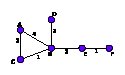
\includegraphics[width=0.5\textwidth]{images/centralities-weighted.pdf}
	\caption{}
	\label{fig:centralities-weighted}
\end{figure}
First, we compute the Laplacian energy $E(G)$ of the graph as follows:
\begin{eqnarray*}
E_L(G) &=& \sum_{i=1}^n x_i^2 + 2 \sum_{i<j} w_{i,j}^2 \\
&=& (6^2 + 3^2 + 9^2 + 3^2 + 1^2 +2^2 ) + 2 (4^2+2^2+1^2+2^2+2+1^2) \\
&=& 200
\end{eqnarray*}

\begin{table}[H]
	\centering
	\caption{Laplacian Centralities of edges}
	%\setlength{\tabcolsep}{16pt}
	%\scalebox{0.7}{
		\begin{tabular}{|l| c|c|c|}
			\hline 
		Edge(e) & $E(H);H=G-e$ & $E(G)-E(H)$ & $\Delta(E)$ by walks method in (\ref{walksenergyeqn}) \\
		\hline
		a,c & 164 & $200-164 = 36$ & $2(2) + 2(8) +4(4) = 36$ \\
		b,c & 176 & $200-176 = 24$ & $2(2+2+4) + 2(2) + 4(1) = 24$ \\
		a,b & 80 & $200-80 = 120$ & $2(8)+ 2(4+8+8) + 2(16) = 120$ \\
		b,d & 156 & $200-156 = 44$ & $2(0) + 2(4+8+2) +4(4)=44$
		\\
		b,e & 152 & $200-158 =88$ & $2(2) + 2(4+8+2)+ 4(4) = 48$ 
		\\
		e,f & 192 & $200-192 = 8$ & $2(0) + 2(2)+ 4(1) = 8$\\
		\hline
		\end{tabular}
	\label{edgelaptab}
\end{table}

\end{exa}
From Table \ref{edgelaptab}, we observe the drop in energy 
computed by the difference between Laplacian energy of the graph $G$ and that of the subgraph, $H$ obtained on removing edge $e$ is equal to that obtained using closed and non-closed walks in  (\ref{walksenergyeqn}).

\subsection{Laplacian Energy as a fair measure of robustness of network}
With the fast increasing usage of air transport in most regions of the world, there is a pressing need to design robust air traffic networks that will ensure robustness when one or more flights are removed or added to the network. The second smallest eigenvalue of the Laplacian matrix of air traffic networks, $\lambda_2$, also known as the algebraic connectivity is a common measure of robustness in networks. Unfortunately, the algebraic connectivity captures only the global information about the connectivity of a network.
Recently, the laplacian energy was introduced as another measure of robustness that is considered fair and effective compared to the algebraic connectivity. This is so because the Laplacian centrality captures the local information of the network (Yang,etal, 2015). 
In order to illustrate the relationship between Laplacian energy and air traffic network
robustness, a real air traffic network of Jet-star Asia Airway among Indonesia, Australia,
and New Zealand (Fig.~\ref{jetstarnetwork} ) was investigated.


\begin{figure}[!h]
	\centering
	\begin{subfigure}[b]{0.45\textwidth}
		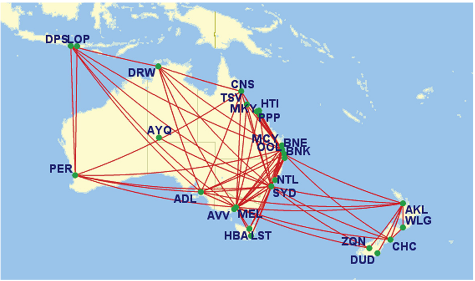
\includegraphics[width=\textwidth]{images/jetstar-airnetwork.png}
		\caption{}
		\label{jetstarnetwork}
	\end{subfigure}~
	\begin{subfigure}[b]{0.45\textwidth}
		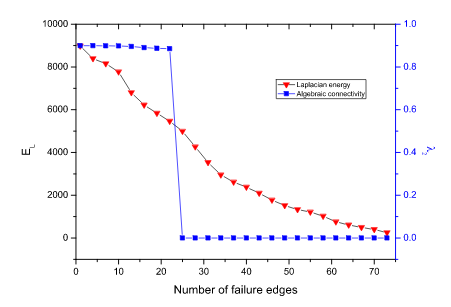
\includegraphics[width= \textwidth]{images/lapalgebraic.png}
		\caption{}
		\label{connectivitycurve}
	\end{subfigure}
	\caption{(\subref{jetstarnetwork}) is the air traffic network route map for Jetstar Asia Airway (Indonesia, Australia, and New Zealand) in 2015,  (\subref{connectivitycurve}) is a plot of Laplacian energy $E_L$ and algebraic connectivity $\lambda_2$ against the number of randomly failed edges from the or Jetstar Asia Airway (Indonesia, Australia, and New Zealand). }
	\label{robustness}
\end{figure}




From the Fig.~(\ref{connectivitycurve}), we observe that values for both the laplacian energy and algebraic connectivity decreases with removal of edges from the network. However, on removal of $20$ to $30$ edges, the algebraic connectivity abruptly drops from $0.9$ to close to $0$ (that is in only one instance) which signifies a disconnection in the network that is, more than one connected component in the network. on the other hand though, the laplacian curve indicates gradual degradation of the network robustness on removal of $20$ to $30$ edges of the network. The ability of the Laplacian energy measure to capture the change from one connected component to more connected components in much more instances makes it an effective measure for network robustness over algebraic connectivity.

\renewcommand{\bibname}{References}
\nocite{*}
\bibliographystyle{abbrvnat}
\bibliography{references}

\end{document}